% Options for packages loaded elsewhere
\PassOptionsToPackage{unicode}{hyperref}
\PassOptionsToPackage{hyphens}{url}
\PassOptionsToPackage{dvipsnames,svgnames*,x11names*}{xcolor}
%
\documentclass[
  11pt,
]{article}
\usepackage{lmodern}
\usepackage{amssymb,amsmath}
\usepackage{ifxetex,ifluatex}
\ifnum 0\ifxetex 1\fi\ifluatex 1\fi=0 % if pdftex
  \usepackage[T1]{fontenc}
  \usepackage[utf8]{inputenc}
  \usepackage{textcomp} % provide euro and other symbols
\else % if luatex or xetex
  \usepackage{unicode-math}
  \defaultfontfeatures{Scale=MatchLowercase}
  \defaultfontfeatures[\rmfamily]{Ligatures=TeX,Scale=1}
\fi
% Use upquote if available, for straight quotes in verbatim environments
\IfFileExists{upquote.sty}{\usepackage{upquote}}{}
\IfFileExists{microtype.sty}{% use microtype if available
  \usepackage[]{microtype}
  \UseMicrotypeSet[protrusion]{basicmath} % disable protrusion for tt fonts
}{}
\makeatletter
\@ifundefined{KOMAClassName}{% if non-KOMA class
  \IfFileExists{parskip.sty}{%
    \usepackage{parskip}
  }{% else
    \setlength{\parindent}{0pt}
    \setlength{\parskip}{6pt plus 2pt minus 1pt}}
}{% if KOMA class
  \KOMAoptions{parskip=half}}
\makeatother
\usepackage{xcolor}
\IfFileExists{xurl.sty}{\usepackage{xurl}}{} % add URL line breaks if available
\IfFileExists{bookmark.sty}{\usepackage{bookmark}}{
\usepackage{hyperref}
}
\hypersetup{
  pdftitle={TP table de données, fusion},
  pdfauthor={Première NSI Lycée du Parc},
  colorlinks=true,
  linkcolor=Maroon,
  filecolor=Maroon,
  citecolor=Blue,
  urlcolor=Blue,
  pdfcreator={LaTeX via pandoc}}
\urlstyle{same} % disable monospaced font for URLs
\usepackage[top=20mm,left=20mm,right=20mm,heightrounded]{geometry}
\usepackage{listings}
\newcommand{\passthrough}[1]{#1}
\lstset{defaultdialect=[5.3]Lua}
\lstset{defaultdialect=[x86masm]Assembler}
\usepackage{graphicx}
\makeatletter
\def\maxwidth{\ifdim\Gin@nat@width>\linewidth\linewidth\else\Gin@nat@width\fi}
\def\maxheight{\ifdim\Gin@nat@height>\textheight\textheight\else\Gin@nat@height\fi}
\makeatother
% Scale images if necessary, so that they will not overflow the page
% margins by default, and it is still possible to overwrite the defaults
% using explicit options in \includegraphics[width, height, ...]{}
\setkeys{Gin}{width=\maxwidth,height=\maxheight,keepaspectratio}
% Set default figure placement to htbp
\makeatletter
\def\fps@figure{htbp}
\makeatother
\setlength{\emergencystretch}{3em} % prevent overfull lines
\providecommand{\tightlist}{%
  \setlength{\itemsep}{0pt}\setlength{\parskip}{0pt}}
\setcounter{secnumdepth}{5}

\title{TP table de données, fusion}
\usepackage{etoolbox}
\makeatletter
\providecommand{\subtitle}[1]{% add subtitle to \maketitle
  \apptocmd{\@title}{\par {\large #1 \par}}{}{}
}
\makeatother
\subtitle{Traitement de données en tables}
\author{Première NSI Lycée du Parc}
\date{}

%%%jolis boites

\usepackage{fancybox, graphicx}



%%%%%%%%%%%%%%%%Packages et Macros Frederic%%%%%%%%%%%%%%%%%%%%%%%%%%%%%


%%%%Insertion de liens hypertextes %%%%

            
%%%%%%%%%%PSTricks%%%%%%%%%%%%

\usepackage{pstricks,pst-plot,pst-text,pst-tree,pst-eps,pst-fill,pst-node,pst-math,pstricks-add,pst-xkey,pst-eucl}


%%%%%%%Tikz%%%%%%%%%%%%%%%
\usepackage{pgf,tikz,tkz-tab}
% Pour les tableaux de signes ou de variations avec tkz-tab voir https://zestedesavoir.com/tutoriels/439/des-tableaux-de-variations-et-de-signes-avec-latex/#1-13389_tikz-un-package-qui-en-a-dans-le-ventre
\usetikzlibrary{arrows}
\usetikzlibrary{shapes.geometric}
\usetikzlibrary{shapes.geometric}
\usetikzlibrary{petri}
\usetikzlibrary{decorations}
\usetikzlibrary{arrows}
\usetikzlibrary{math}
 %Variables must be declared in a tikzmath environment but
       % can be used outside
%       \tikzmath{int \n; \n = 508; \x1 = 1; \y1 =1; 
%                   %computations are also possible
%                    \x2 = \x1 + 1; \y2 =\y1 +3; } 


%%%%%%%%%%%%%%%%%%%%%%%%%%%%%%%%%%%%%%%%
%%%%%%%%%%%Commandes Tikz Perso%%%%%%%%%%%%%%%

% Définition des nouvelles options xmin, xmax, ymin, ymax
% Valeurs par défaut : -3, 3, -3, 3
\tikzset{
xmin/.store in=\xmin, xmin/.default=-3, xmin=-3,
xmax/.store in=\xmax, xmax/.default=3, xmax=3,
ymin/.store in=\ymin, ymin/.default=-3, ymin=-3,
ymax/.store in=\ymax, ymax/.default=3, ymax=3,
}
% Commande qui trace la grille entre (xmin,ymin) et (xmax,ymax)
\newcommand {\grille}[2]
{\draw[help lines,black, thick] (\xmin,\ymin) grid[xstep=#1, ystep=#2] (\xmax,\ymax);}
% Commande \axes
\newcommand {\axes} {
\draw[->,very thick] (\xmin,0) -- (\xmax,0);
\draw[->,very thick] (0,\ymin) -- (0,\ymax);
\draw (0.95*\xmax, 0) node[above] {};
\draw (0, 0.95*\ymax) node[left] {};
}
% Commande qui limite l?affichage à (xmin,ymin) et (xmax,ymax)
\newcommand {\fenetre}
{\clip (\xmin,\ymin) rectangle (\xmax,\ymax);}

%Exemple d'utilisation

%\begin{center}
%\begin{tikzpicture} [xmin=-2,xmax=2,ymin=0,ymax=5]
%\grille{1} \axes \fenetre
%\draw plot[smooth] (\x,\x^2);
%\end{tikzpicture}
%\end{center}

%style pour la perspective cavalière française
%voir Tikz pour l'impatient page 68
\tikzset{math3d/.style=
{x= {(-0.353cm,-0.353cm)}, z={(0cm,1cm)},y={(1cm,0cm)}}}

%%%%%%%Symbole pour code calculatrice%%%%%%

%Flèche remplie pour défilement de menu

\newcommand{\flechefillright}{

\begin{tikzpicture}[scale=0.15] \fill (0,0)--(2,1)--(0,2)--cycle;
\end{tikzpicture}}

%%%%%%%%%%%%%Symboles pour calculatrice Casio%%%%
\newcommand{\execasio}{\Pisymbol{psy}{191}} %Retour chariot
\newcommand{\dispcasio}{\begin{pspicture}(.1,.1)\pspolygon*(.1,0)(.1,.1)\end{pspicture}} %Triangle « Disp »
\newcommand{\dispcasiotikz}{
\begin{tikzpicture}[scale=0.2]
\fill (0,0) -- (1,0) -- (1,1) -- cycle;
\end{tikzpicture}} %Triangle « Disp »
%

%Fleche entre deux lignes, d'apres 'un bon petit' : http://forum.mathematex.net/latex-f6/fleches-entre-deux-lignes-pour-resolution-d-equation-t10283.html#p99817
\newcommand\addnode[1]{\Rnode{#1}{}}
\newcommand\linknode[3]{\ncbar[angleA=0,angleB=0,nodesep=1ex,arm=10ex,offset=-2pt]{->}{#1}{#2}\Aput{\vphantom{x}#3}}


%%Commande pour touche de calculatrice

\newcommand\tc[1]{%
{
\begin{tikzpicture}
\node[draw,rectangle,rounded corners=3pt] (P) at (0,0){#1};
\end{tikzpicture}
}
}

%%%%%%%%%%%%%%%%%%%%%%%%%%%%%%%%%%%%%%%%
%%%%%%%%%%%Fin Commandes Tikz%%%%%%%%%%%%%%%


%%%%%%%%%%%%Specifiques%%%%%%%%%%%
\usepackage{wrapfig}
%pour insérer une figure à droite ou à gauche d'un texte
%\begin{wrapfigure}[nb lignes]{placement l,r,c,i(inside),o(outside)}[overhang]{width}
%ce package fonctionne mal à proximité des listes
%%%%%%%%%%%%%%%%%%%%%%%%%%%%%%%%%%%%%

%%%%%Environnements et symboles spéciaux pour faire joli%%%%%%

%%%Bclogo, pour des environnements + jolis avec insertion de logo%%%%
%Dépendances de  bclogo
\usepackage{xkeyval}  
\usepackage{etoolbox}
\usepackage{ifpdf}
\usepackage[framemethod=tikz]{mdframed}
\usepackage[tikz]{bclogo}

%\newcommand\bcpython{
\includegraphics[width=17pt]{/home/fjunier/Maths/python-logo.eps}}
\newcommand\bcpython{
\includegraphics[width=17pt]{/home/fjunier/Maths/python-logo.png}}
%\newcommand\bcpython{
\includegraphics[width=17pt]{/home/frederic/Maths/python-logo.png}}

%% Framed
\usepackage{framed}  %Le package « framed» Crée 3 nouveaux environnements, qui se comportent comme des minipage de largeur \linewidth, mais permettant en plus de se casser entre plusieurs pages.     * framed : avec un cadre autour;     * shaded : avec un fonc coloré (il faut définir la couleur shadecolor);     * leftbar : avec une barre le long du côté gauche.

%%%%%%%%%%%%%%%%%%%Présentation de codes sources%%%%%%%%%%%%%%%%%
\usepackage{listings}
%On utilise l?environnement lstlisting pour insérer
%un code source.
%En plus de l?environnement lstlisting, on peut également utiliser la
%commande \lstinline qui fonctionne comme la commande \verb, en ce
%sens qu?on peut utiliser n?importe quel caractère comme délimiteur. Enfin,
%la commande \lstinputlisting permet de charger un code source depuis
%un fichier externe.
%Il y a deux manières de préciser des options : soit via l?option de l?envi-
%ronnement ou de la commande, soit en utilisant la commande \lstset
%qui permet de définir des options de manière globale.

\lstset{ %
  language=Python,                % the language of the code
  basicstyle=\ttfamily,           % the size of the fonts that are used for the code
  %numbers=left,                   % where to put the line-numbers
  numberstyle=\tiny,  % the style that is used for the line-numbers
  %stepnumber=2,                   % the step between two line-numbers. If it's 1, each line 
                                  % will be numbered
  %numbersep=5pt,                  % how far the line-numbers are from the code
  backgroundcolor=\color{white},      % choose the background color. You must add \usepackage{color}
  showspaces=false,               % show spaces adding particular underscores
  showstringspaces=false,         % underline spaces within strings
  showtabs=false,                 % show tabs within strings adding particular underscores
  frame=single,                   % adds a frame around the code
  rulecolor=\color{black},        % if not set, the frame-color may be changed on line-breaks within not-black text (e.g. comments (green here))
  tabsize=4,                      % sets default tabsize to 2 spaces
  captionpos=b,                   % sets the caption-position to bottom
  breaklines=true,                % sets automatic line breaking
  breakatwhitespace=false,        % sets if automatic breaks should only happen at whitespace
  %title=\lstname,                   % show the filename of files included with \lstinputlisting;
                                  % also try caption instead of title
  breakindent=1cm,
  keywordstyle=\color{blue},          % keyword style
  commentstyle=\color{red},       % comment style
  %stringstyle=\ttfamily\color{green},         % string literal style
  escapeinside={\%*}{*)},            % if you want to add LaTeX within your code
  morekeywords={*,...},              % if you want to add more keywords to the set
  deletekeywords={...}              % if you want to delete keywords from the given language
  upquote=true,columns=flexible,
xleftmargin=1cm,xrightmargin=1cm,
 inputencoding=utf8,			%Les lignes qui suivent sont pour le codage utf8
  extendedchars=true,
  literate=%
            {é}{{\'{e}}}1
            {è}{{\`{e}}}1
            {ê}{{\^{e}}}1
            {ë}{{\¨{e}}}1
            {û}{{\^{u}}}1
            {ù}{{\`{u}}}1
            {â}{{\^{a}}}1
            {à}{{\`{a} }}1
            {î}{{\^{i}}}1
            {ô}{{\^{o}}}1
            {ç}{{\c{c}}}1
            {Ç}{{\c{C}}}1
            {É}{{\'{E}}}1
            {Ê}{{\^{E}}}1
            {À}{{\`{A}}}1
            {Â}{{\^{A}}}1
            {Î}{{\^{I}}}1
}

\lstdefinestyle{rond}{
  numbers=none,
  backgroundcolor=\color{gristclair},
  frameround =tttt
}

\lstdefinestyle{compil}{
  numbers=none,
  backgroundcolor=\color{gristclair}
}
%\lstset{language=Python,basicstyle=\small , frame=single,tabsize=4,showspaces=false,showtabs=false,showstringspaces=false,numbers=left,numberstyle=\tiny , extendedchars=true}



%%%%%%%%%%%%%%%%%%%%%%%%%%%%%%%%%%%%%%%%%%%%%%%%%%%%%%%%%%%%%%%%%%%%%%%%
%%%%%%%%%%%%%%%%%%%%Environnements persos%%%%%%%%%%%%%%%%%%%%%%%%%%%%%%%%
%Syntaxe :
%\newenvironment{nom}[nombre d'args][defaut]{definitions initiales}{definitions finales}
%definitions intiales sont les commandes appelées par \begin{nom}
%Definitions finales sont les commandes appelées par \end{nom}

%%%%%%%%%%%%%%%%Définitions des environnemts persostheoreme, exemple ..%%%%
%%%% Exercice avec encadré %%%%
\newcounter{exo}
\newenvironment{exercice}[1]
{\par \medskip   \addtocounter{exo}{1} \noindent  
\begin{bclogo}[arrondi =0.1,   noborder = true, logo=\bccrayon, marge=4]{~\textbf{Exercice} \textbf{\theexo} {\itshape #1} }  \par}
{
\end{bclogo}
 \par \bigskip }

%%Axiomes, Theoremes, Propriété, Définition, Methode, Preuve


\newenvironment{axiome}[1]
{\par \medskip   \begin{leftbar} \noindent \underline{\textbf{Axiome}}\hspace{0.5cm}{\itshape #1}   \vspace*{10pt} \par }
{\end{leftbar}  \par \medskip }


\newcounter{thme}
\newenvironment{theoreme}[1]
{\par \medskip  \addtocounter{thme}{1} \noindent  
\begin{bclogo}[arrondi =0.1,  ombre = true, barre=none, logo=\bcbook, marge=4]{~\textbf{Théorème} \textbf{\thethme} {\itshape #1} }   \par}
{
\end{bclogo}
 \par \bigskip}

 \newenvironment{theoremedef}[1]
{\par \medskip   \addtocounter{thme}{1} \noindent  
\begin{bclogo}[arrondi =0.1,  ombre = true, barre=none, logo=\bcbook, marge=4]{~\textbf{Théorème-Définition} \textbf{\thethme} {\itshape #1} }   \par}
{
\end{bclogo}
 \par \bigskip }
 
\newcounter{prop}
\newenvironment{propriete}[1]
{\par \medskip   \addtocounter{prop}{1} \noindent  
\begin{bclogo}[arrondi =0.1,  ombre = true, barre=none, logo=\bcbook, marge=4]{~\textbf{Propriété} \textbf{\theprop} {\itshape #1} }   \par}
{
\end{bclogo}
 \par \bigskip }


\newenvironment{corollaire}[1]
{\par \medskip   \noindent  
\begin{bclogo}[arrondi =0.1,  ombre = true, barre=none, logo=\bcbook, marge=4]{~\textbf{Corollaire} {\itshape #1} } \par }
{
\end{bclogo}
 \par \bigskip }

\newenvironment{demo}[1]
{\par \medskip   \noindent  
\begin{bclogo}[arrondi =0.1,  ombre = true, barre=zigzag, noborder = true, logo=\bcloupe, marge=0]{~\textbf{Démonstration} {\itshape #1} } \par \vspace{10pt}}
{
\end{bclogo}
 \par \bigskip }

\newcounter{activite}
\newenvironment{activite}[1]
{\par \medskip   \noindent   \addtocounter{activite}{1}
\begin{bclogo}[arrondi =0.1,   noborder = true, logo=\bcvelo, marge=4]{~\textbf{Activité} \textbf{\theactivite} {\itshape #1} }  \par}
{
\end{bclogo}
 \par \bigskip }


\newenvironment{synthese}
{\par \medskip   \noindent   
\begin{bclogo}[arrondi =0.1,   noborder = true, logo=\bccle, marge=4]{~\textbf{Synthèse}   }  \par}
{
\end{bclogo}
 \par \bigskip }
 
 
\newcounter{rque}
\newenvironment{remarque}
{\par \medskip    \addtocounter{rque}{1} \noindent  
\begin{bclogo}[arrondi =0.1,  ombre = true, barre=snake, noborder = true, logo=\bcinfo, marge=0]{~\textbf{Remarque} \textbf{\therque}}  \par }
{
\end{bclogo}
 \par \bigskip }

\newcounter{def}
\newenvironment{definition}[1]
{\par \medskip   \addtocounter{def}{1} \noindent  
\begin{bclogo}[arrondi =0.1,  ombre = true, barre=none, logo=\bcbook, marge=4]{~\textbf{Définition} \textbf{\thedef} {\itshape #1} }  \par}
{
\end{bclogo}
 \par \bigskip }
 
 
 \newcounter{cours}
\newenvironment{cours}[1]
{\par \medskip   \addtocounter{cours}{1} \noindent  
\begin{bclogo}[arrondi =0.1,  ombre = true, barre=none, logo=\bcbook, marge=4]{~\textbf{Point de cours} \textbf{\thecours} {\itshape #1} }  \par}
{
\end{bclogo}
 \par \bigskip }
 
 

\newenvironment{introduction}
{\par \medskip    \noindent  
 \begin {bclogo}[couleur = blue!5 , arrondi =0.1,logo=\bcrosevents, marge=4] {~\textbf{Introduction}    }
 \par }
{
\end{bclogo}
 \par \bigskip }
 
\newenvironment{memo}[1]
{\par \medskip    \noindent  
\begin{bclogo}[arrondi =0.1,  ombre = true, barre=none, logo=\bccle, marge=4]{~\textbf{À retenir}  {\itshape #1} }  \par}
{
\end{bclogo}
 \par \bigskip }
 
\newcounter{exple}
\newenvironment{exemple}[1]
{\par \medskip   \addtocounter{exple}{1} \noindent  
\begin{bclogo}[arrondi =0.1,   noborder = true, logo=\bclampe, marge=4]{~\textbf{Exemple} \textbf{\theexple} {\itshape #1} }  \par}
{
\end{bclogo}
 \par \bigskip }




\newcounter{alg}
\newenvironment{algorithme}[1]
{\par \medskip   \addtocounter{alg}{1} \noindent  
 \begin {bclogo}[noborder = true, barre=zigzag,logo=\bcpython, marge=4] {~\textbf{Algorithmique} \textbf{\thealg} {\itshape #1} }  \par}
{
\end{bclogo}
 \par \bigskip }

\newcounter{prog}
\newenvironment{programme}[1]
{\par \medskip   \addtocounter{prog}{1} \noindent  
 \begin {bclogo}[noborder = true, barre=zigzag,logo=\bcpython, marge=4] {~\textbf{Programme} \textbf{\theprog} {\itshape #1} }  \par  \bigskip}
{
\end{bclogo}
 \par \bigskip }
 
\newcounter{logi}
\newenvironment{logique}[1]
{\par \medskip   \addtocounter{logi}{1} \noindent  
 \begin {bclogo}[noborder = true, barre=zigzag,logo=\bclampe, marge=4] {~\textbf{Logique} \textbf{\thelogi} {\itshape #1} }  \par}
{
\end{bclogo}
 \par \bigskip }


\newenvironment{methode}[1]
{\par \medskip    \noindent  
 \begin {bclogo}[arrondi =0.1,logo=\bcoutil, marge=4,noborder = true] {~\textbf{Méthode}   {\itshape #1} }  \par}
{
\end{bclogo}
 \par \bigskip }


\newcounter{histo}
\newenvironment{histoire}[1]
{\par \medskip   \addtocounter{histo}{1} \noindent  
 \begin {bclogo}[couleur = blue!10 , arrondi =0.1,logo=\bchorloge, marge=4] {~\textbf{Histoire} \textbf{\thehisto} {\itshape #1} }  \par}
{
\end{bclogo}
 \par \bigskip }




%Environnement contenu pour un document présentant une progression annuelle
\newenvironment{contenu}
{\par \medskip   \begin {bclogo}[ noborder = true,logo=\bccrayon] \noindent {\large \textbf{Contenu de la séance}} \vspace*{10pt} \par  }
{\end{bclogo}  \par \medskip }

%Environnement programme pour un document présentant une progression annuelle
%\newenvironment{programme}
%{\par \medskip   \begin {bclogo}[ noborder = true, barre=zigzag,logo=\bcinfo] \noindent {\large \textbf{Programme officiel}} \vspace*{10pt} \par  }
%{\end{bclogo}  \par \medskip }

%Environnement programme pour un document présentant une progression annuelle
\newenvironment{ressource}
{\par \medskip   \begin {bclogo}[ noborder = true,logo=\bcbook] \noindent {\large \textbf{Ressources}}\\vspace*{10pt} \par }
{\end{bclogo}  \par \medskip }




%%%%%%%%%%%%%%%%%%Maths divers%%%%%%%%%%%%%%%%%%%%%%%%%
%%%%%%%%%%%%%Nombres%%%%%%%%%%%%%%%%

%Ensemble prive de...
%\newcommand{\prive}{\boi}%{\backslash}

%Ensembles de nombres%%%%%%%%%%%%%%%%%
\newcommand{\R}{\mathbb{R}}
\newcommand{\N}{\mathbb{N}}
\newcommand{\D}{\mathbb{D}}
\newcommand{\Z}{\mathbb{Z}}
\newcommand{\Q}{\mathbb{Q}}
%\newcommand{\C}{\mathbb{C}}
\newcommand{\df}{~\ensuremath{]0;+\infty[}~}
\newcommand{\K}{\mathbb{K}}

%%%%%%%%Arithmetique%%%%%%%%%%
%PGCD, PPCM
\newcommand{\PGCD}{\mathop{\rm PGCD}\nolimits}
\newcommand{\PPCM}{\mathop{\rm PPCM}\nolimits}

%Intervalles
\newcommand{\interoo}[2]{]#1\, ;\, #2[}
\newcommand{\Interoo}[2]{\left]#1\, ;\, #2\right[}
\newcommand{\interof}[2]{]#1\, ;\, #2]}
\newcommand{\Interof}[2]{\left]#1\, ;\, #2\right]}
\newcommand{\interfo}[2]{[#1\, ;\, #2[}
\newcommand{\Interfo}[2]{\left[#1\, ;\, #2\right[}
\newcommand{\interff}[2]{[#1\, ;\, #2]}
\newcommand{\Interff}[2]{\left[#1\, ;\, #2\right]}
%\newcommand\interentiers #1#2{[\! [#1\, ;\, #2]\! ]}
\newcommand{\interentiers}[2]{\llbracket #1\, ;\, #2\rrbracket}
%


%%%%%%%%%%%%%%Nombres complexes%%%%%

\newcommand{\ic}{\text{i}}
%\newcommand{\I}{\text{i}}
\newcommand{\im}[1]{\text{Im}\left(#1\right)}
\newcommand{\re}[1]{\text{Re}\left(#1\right)}
\newcommand{\Arg}[1]{\text{arg}\left(#1\right)}
\newcommand{\Mod}[1]{\left[#1\right]}
%Parties entière, réelle, imaginaire, nombre i
\newcommand{\ent}[1]{\text{E}\left(#1\right)}
\renewcommand{\Re}{\mathop{\rm Re}\nolimits}
\renewcommand{\Im}{\mathop{\rm Im}\nolimits}
\renewcommand{\i}{\textrm{i}}

%%%%%%%%%%%Probabilites et statistiques%%%%%
\newcommand{\loibinom}[2]{\mathcal{B}\left(#1\ ; \ #2 \right)}
\newcommand{\loinorm}[2]{\mathcal{N}\left(#1\ ; \ #2 \right)}
\newcommand{\loiexp}[1]{\mathcal{E}\left(#1\right)}
\newcommand{\proba}[1]{\mathbb{P}\big(#1\big)}
\newcommand{\probacond}[2]{\mathbb{P}_{#2}\big(#1\big)}
\newcommand{\esperance}[1]{\mathbb{E}\left(#1\right)}
\newcommand{\variance}[1]{\mathbb{V}\left(#1\right)}
\newcommand{\ecart}[1]{\sigma\left(#1\right)}
\newcommand{\dnormx}{\frac{1}{\sqrt{2\pi}} \text{e}^{-\frac{x^2}{2}}}
\newcommand{\dnormt}{\frac{1}{\sqrt{2\pi}} \text{e}^{-\frac{t^2}{2}}}

%Covariance
\newcommand{\cov}{\mathop{\rm cov}\nolimits}
%


%%%%%%%%%%Analyse%%%%%%%%%%%

%%%%%%%%%%%Courbe%%%%%%%%%%%%
\newcommand{\courbe}[1]{\ensuremath{\mathcal{C}_{#1}}}

%%%%%%%Fonction exponentielle%%%%%
\newcommand{\fe}{~fonction exponentielle~}
\newcommand{\e}{\text{e}}

%Fonction cotangente
\newcommand{\cotan}{\mathop{\rm cotan}\nolimits}
%%%%%%%%%%%%%%%%%%%%%%%%%%%%%%%%%%%%%%%%%
%
%Fonctions hyperboliques
\newcommand{\ch}{\mathop{\rm ch}\nolimits}
\newcommand{\sh}{\mathop{\rm sh}\nolimits}


%%%%%%%%%%%%%%Limites%%%%%%
\newcommand{\limite}[2]{\lim\limits
_{x \to #1} #2}
\newcommand{\limitesuite}[1]{\lim\limits
_{n \to +\infty} #1}
\newcommand{\limiteg}[2]{\lim\limits
_{\substack{x \to #1 \\ x < #1 }} #2}
\newcommand{\limited}[2]{\lim\limits
_{\substack{x \to #1 \\ x > #1 }} #2}

%%%%%%%%%%Continuité%%%%%%%%%%%
\newcommand{\TVI}{théorème des valeurs intermédiaires}

%%%%%%%%%%%Suites%%%%%%%%%%%%
\newcommand{\suite}[1]{\ensuremath{\left(#1_{n}\right)}}
\newcommand{\Suite}[2]{\ensuremath{\left(#1\right)_{#2}}}
%

%%%%%%%%%%%%%%%Calcul intégral%%%%%%
\newcommand{\dx}{\ensuremath{\text{d}x}}		% dx
\newcommand{\dt}{\ensuremath{\text{d}t}}		% dt
\newcommand{\dtheta}{\ensuremath{\text{d}\theta}}		% dtheta
\newcommand{\dy}{\ensuremath{\text{d}y}}		% dy
\newcommand{\dq}{\ensuremath{\text{d}q}}		% dq

%%%Intégrale%%%
\newcommand{\integralex}[3]{\int_{#1}^{#2} #3 \ \dx}
\newcommand{\integralet}[3]{\int_{#1}^{#2} #3 \ \dt}
\newcommand{\integraletheta}[3]{\int_{#1}^{#2} #3 \ \dtheta}

%%%%%Equivalent%%
\newcommand{\equivalent}[1]{\build\sim_{#1}^{}}

%o et O%%%%
\renewcommand{\o}[2]{\build o_{#1\to #2}^{}}
\renewcommand{\O}[2]{\build O_{#1\to #2}^{}}



%%%%%%%%%%%%%%%Geometrie%%%%%%%%%%%%%%%%%%%%%%%

%%%%%%%%%%%%%%%Reperes%%%%%%%%%%%%%%
\def\Oij{\ensuremath{\left(\text{O},~\vect{\imath},~\vect{\jmath}\right)}}
\def\Oijk{\ensuremath{\left(\text{O},~\vect{\imath},~ \vect{\jmath},~ \vect{k}\right)}}
\def\Ouv{\ensuremath{\left(\text{O},~\vect{u},~\vect{v}\right)}}
\renewcommand{\ij}{(\vec\imath\, ;\vec\jmath\,)}
\newcommand{\ijk}{(\vec\imath\, ;\vec\jmath\, ;\vec k\,)}
\newcommand{\OIJ}{(O\,;\, I\,;\, J\,)}
\newcommand{\repere}[3]{\big(#1\, ;\,\vect{#2} ;\vect{#3}\big)}
\newcommand{\reperesp}[4]{\big(#1\, ;\,\vect{#2} ;\vect{#3} ;\vect{#4}\big)}

%%%%%%%%%Coordonnees%%%%%%%%%%%%%%
\newcommand{\coord}[2]{(#1\, ;\, #2)}
\newcommand{\bigcoord}[2]{\big(#1\, ;\, #2\big)}
\newcommand{\Coord}[2]{\left(#1\, ;\, #2\right)}
\newcommand{\coordesp}[3]{(#1\, ;\, #2\, ;\, #3)}
\newcommand{\bigcoordesp}[3]{\big(#1\, ;\, #2\, ;\, #3\big)}
\newcommand{\Coordesp}[3]{\left(#1\, ;\, #2\, ;\, #3\right)}
\newcommand{\Vcoord}[3]{\begin{pmatrix} #1 \\ #2 \\ #3 \end{pmatrix}}
%Symboles entre droites
%\newcommand{\paral}{\sslash}
\newcommand{\paral}{\mathop{/\!\! /}}
%

%%%%%%%%%Produit scalaire, Angles%%%%%%%%%%
\newcommand{\scal}[2]{\vect{#1} \, \cdot \, \vect{#2}}
\newcommand{\Angle}[2]{\left(\vect{#1} \, , \, \vect{#2}\right)}
\newcommand{\Anglegeo}[2]{\left(\widehat{\vect{#1} \, ; \, \vect{#2}}\right)}
\renewcommand{\angle}[1]{\widehat{#1}}
\newcommand{\anglevec}[2]{\left(\vect {#1}\, ,\,\vect {#2} \right)}
\newcommand{\anglevecteur}[2]{(#1\, , \, #2)}
\newcommand{\Anglevec}[2]{(\vecteur{#1}\, ,\,\vecteur{#2})}
\newcommand{\prodscal}[2]{#1 \, \cdot \, #2}
%


%Arc
%\newcommand{\arc}[1]{\wideparen{#1}}
\newcommand{\arcoriente}[1]{\overset{\curvearrowright}{#1}}
%
%


%%%%%%%%%%%%%%%Normes%%%%%%%%%%%%%%%%
\newcommand{\norme}[1]{\left\| #1\right\|}
\newcommand{\normebis}[1]{\delim{2pt}{\|}{9pt}\! #1\delim{2pt}{\|}{9pt}}
\newcommand{\normetriple}[1]{\left |\kern -.07em\left\| #1\right |\kern -.07em\right\|}
\newcommand{\valabs}[1]{\big| \, #1 \, \big|}
%

%%%%%%%%%%%%%%%%%%%%%%%%%%%Degré%%%%%%
%\newcommand{\Degre}{\ensuremath{^\circ}}
%La commande \degre est déjà définie dans le package babel

%%%%%%%%%%Vecteurs%%%%%%%%%%%
\newcommand{\vect}[1]{\mathchoice%
{\overrightarrow{\displaystyle\mathstrut#1\,\,}}%
{\overrightarrow{\textstyle\mathstrut#1\,\,}}%
{\overrightarrow{\scriptstyle\mathstrut#1\,\,}}%
{\overrightarrow{\scriptscriptstyle\mathstrut#1\,\,}}}



%%%%%%%%%%%%%Algebre%%%%%%%%%%%%%%%


%%%%%%%%%%Systemes%%%%%%%%%%%
%Systemes
\newcommand{\sys}[2]{
\left\lbrace
 \begin{array}{l}
  \negthickspace\negthickspace #1\\
  \negthickspace\negthickspace #2\\
 \end{array}
\right.\negthickspace\negthickspace}
\newcommand{\Sys}[3]{
\left\lbrace
 \begin{array}{l}
  #1\\
  #2\\
  #3\\
 \end{array}
\right.}
\newcommand{\Sysq}[4]{
\left\lbrace
 \begin{array}{l}
  #1\\
  #2\\
  #3\\
  #4\\
 \end{array}
\right.}
%
%

%%%%%%%%%%%%%%%%Matrices%%%%%%%%%%%%%%%%%%
%Comatrice
\newcommand{\com}{\mathop{\rm com}\nolimits}
%
%
%Trace
\newcommand{\tr}{\mathop{\rm tr}\nolimits}
%
%
%Transposee
\newcommand{\transposee}[1]{{\vphantom{#1}}^t\negmedspace #1}
%
%
%Noyau
\newcommand{\Ker}{\mathop{\rm Ker}\nolimits}
%
%

%
%Matrices
\newcommand{\Mn}{\mathcal M_n}
\newcommand{\matrice}[4]{
\left(
 \begin{array}{cc}
  #1 & #2 \\
  #3 & #4
 \end{array}
\right)}

\newcommand{\Matrice}[9]{
\left(
 \begin{array}{ccc}
  #1 & #2 & #3\\
  #4 & #5 & #6\\
  #7 & #8 & #9
 \end{array}
\right)}
\newcommand{\Vect}[3]{
\left(\negmedspace
 \begin{array}{c}
  #1\\
  #2\\
  #3
 \end{array}\negmedspace
\right)}
\newcommand{\Ideux}{\matrice{1}{0}{0}{1}}
\newcommand{\Itrois}{\Matrice{1}{0}{0}{0}{1}{0}{0}{0}{1}}
%
%
%Determinants
\newcommand{\determinant}[4]{
\left|
 \begin{array}{cc}
  #1 & #2 \\
  #3 & #4
 \end{array}
\right|}
\newcommand{\Determinant}[9]{
\left|
 \begin{array}{ccc}
  #1 & #2 & #3\\
  #4 & #5 & #6\\
  #7 & #8 & #9
 \end{array}
\right|}

\begin{document}
\maketitle

\renewcommand*\contentsname{Table des matières}
{
\hypersetup{linkcolor=}
\setcounter{tocdepth}{3}
\tableofcontents
}
\hypertarget{cruxe9dits}{%
\section*{Crédits}\label{cruxe9dits}}
\addcontentsline{toc}{section}{Crédits}

\emph{Ce TP est largement inspiré du chapitres 18 du manuel NSI de la
collection Tortue chez Ellipse, auteurs : Ballabonski, Conchon,
Filliatre, N'Guyen ;}

\hypertarget{ruxe9union-de-tables}{%
\section{Réunion de tables}\label{ruxe9union-de-tables}}

\begin{cours}{}

Si on dispose de deux \textbf{tables de données} avec la même structure
(même nombre d'attributs avec noms et domaines de valeurs identiques),
il est possible de les fusionner en construisant leur \textbf{réunion}
dans une même table en concaténant simplement les lignes /
enregistrements.

L'opérateur \passthrough{\lstinline!+!} de concaténation de tableaux
permet de réaliser très simplement cette opération en Python. On donne
ci-dessous un exemple de réunion de tables de notes de différentes
classes à un devoir commun de NSI. Dans un second exemple, on observe
que si les tables n'ont pas la même structure (attributs différents en
noms et en nombre), on peut les concaténer mais on ne peut plus
manipuler le résultat comme une table :

\begin{lstlisting}[language=Python]
>>> premiere1 = [{'élève' : 'Donald', 'note' : 18},{'élève' : 'Ada', 'note' : 20}]
>>> premiere2 = [{'élève' : 'Alan', 'note' : 19},{'élève' : 'Guido', 'note' : 12}]
>>> premiere_reunion = premiere1 + premiere2
>>> premiere_reunion
[{'élève': 'Donald', 'note': 18}, {'élève': 'Ada', 'note': 20}, {'élève': 'Alan', 'note': 19}, {'élève': 'Guido', 'note': 12}]
>>> premiere3 = [{'prénom' : 'Brian', 'nom' :  'Kernighan', 'note' : 14},{'prénom' : 'Linus', 'nom' : 'Torvalds', 'note' : 8}]
>>> premiere_reunion2 = premiere_reunion + premiere3
>>> prenom = [enreg['élève'] for enreg in premiere_reunion2]
Traceback (most recent call last):
......
KeyError: 'élève'
\end{lstlisting}

\end{cours}

\begin{exercice}{}

\begin{enumerate}
\def\labelenumi{\arabic{enumi}.}
\item
  Télécharger sur la page
  \url{https://www.data.gouv.fr/fr/datasets/prenoms-a-rennes/} le
  fichier
  \href{https://www.data.gouv.fr/fr/datasets/r/4b1b72d6-7238-4bda-a5de-ebd72cb058a0}{\passthrough{\lstinline!prenoms\_gf\_rennes\_zip!}}.
  Extraire l'archive, elle contient huit fichiers CSV dont le nom suit
  le format \passthrough{\lstinline!Prénoms2008GF\_Rennes.csv!},
  recensant les prénoms donnés aux enfants nés dans la ville de Rennes
  entre les années 2008 et 2015.
\item
  Ouvrir un fichier au hasard et lister les attributs de ces tables de
  données.
\item
  Ouvrir dans un IDE Python le fichier
  \passthrough{\lstinline!TP\_Fusion\_Eleve.py!} qui contient des
  fonctions \passthrough{\lstinline!lecture\_csv!} et
  \passthrough{\lstinline!ecriture\_csv!} de manipulation de fichiers
  CSV avec le
  \href{https://docs.python.org/fr/3/library/csv.html}{module
  \passthrough{\lstinline!csv!}} et des codes à compléter.

  Charger les tables contenues dans
  \passthrough{\lstinline!Prénoms2011GF\_Rennes.csv!} et
  \passthrough{\lstinline!Prénoms2010GF\_Rennes.csv!} avec l'instruction
  :

\begin{lstlisting}[language=Python]
prenom_11 = lecture_csv('Prénoms2011GF_Rennes.csv', ';', 'ISO8859')
prenom_10 = lecture_csv('Prénoms2010GF_Rennes.csv', ';', 'ISO8859')
\end{lstlisting}

  On peut noter deux paramètres importants dans l'importation d'un
  fichier CSV : le délimiteur facile à déterminer en éditant le fichier
  (ici le symbole \passthrough{\lstinline!';'!}) et l'encodage (ici
  \passthrough{\lstinline!'ISO8859'!}) qui peut être obtenu avec la
  commande \passthrough{\lstinline!file!} sous Linux :

\begin{lstlisting}[language=bash]
fjunier@fjunier:~/TP-Fusion/Ressources$ file Prénoms2008GF_Rennes.csv 
Prénoms2008GF_Rennes.csv: ISO-8859 text, with CRLF line terminators
\end{lstlisting}
\item
  Tester un mauvais paramètre d'encodage en remplaçant
  \passthrough{\lstinline!'ISO8859'!} par
  \passthrough{\lstinline!'utf8'!} dans
  \passthrough{\lstinline!lecture\_csv!}.
\item
  Compléter le code ci-dessous en respectant les spécifications données
  en \passthrough{\lstinline!docstring!} ou commentaires. On donne des
  postconditions pour vérifier les fonctions
  \passthrough{\lstinline!reunion\_table!} et
  \passthrough{\lstinline!prenom\_max!}.
\end{enumerate}

\begin{lstlisting}[language=Python]
def reunion_table(table1, table2):
    """Paramètres : deux tables table1 et table2
    Valeur renvoyée : table  concaténée de table1 et table2"""
    return ........................

def prenom_max(table):
    """Paramètres : table (ou réunion de tables) de prénoms 
    Valeur renvoyée : tuple constitué de l'effectif maximum
        et du tableau des prénoms  les plus fréquents"""
    effectif_max = int(table[0]['NBR'])
    histo = {table[0]['PRN'] : effectif_max}   
    tab_max = [table[0]['PRN']]
    for enreg in table[1:]:
        prenom = enreg['PRN']
        effectif = int(enreg['NBR'])
        if prenom not in histo:
            histo[prenom] = .................
        else:
            histo[prenom] = .................
        if histo[prenom] > effectif_max:
            .......................
            .......................
        elif histo[prenom] == effectif_max:
            .......................
            .......................
    return (effectif_max, tab_max)      

prenom_10_11 = reunion_table(prenom_10, prenom_11)
assert len(prenom_10) + len(prenom_11) == len(prenom_10_11)
#filtrer uniquement les prénoms féminins dans prenom_10_11
prenom_f_10_11 = [enreg for enreg in prenom_10_11 
                 if ................................................]
assert prenom_max(prenom_f_10_11) == (103, ['Louise'])
\end{lstlisting}

\begin{enumerate}
\def\labelenumi{\arabic{enumi}.}
\setcounter{enumi}{5}
\tightlist
\item
  Exécuter le code ci-dessous. Quel point de vigilance lors de la
  réunion de tables est ainsi mis en évidence ?
\end{enumerate}

\begin{lstlisting}[language=Python]
#chargement de deux nouvelles tables
prenom_08 = lecture_csv('Prénoms2008GF_Rennes.csv', ';', 'ISO8859')
prenom_09 = lecture_csv('Prénoms2009GF_Rennes.csv', ';', 'ISO8859')
prenom_08_09 = reunion_table(prenom_08, prenom_09)

def clef_prenom(enreg):
    return enreg['PRN']

def clef_prenom_annee(enreg):
    return (enreg['PRN'], enreg['ANNAISS'])


assert sorted(prenom_09, key = clef_prenom_annee) == sorted(prenom_09, key = clef_prenom)
prenom_08_09_tri = sorted(prenom_08_09, key = clef_prenom_annee) 
\end{lstlisting}

\begin{enumerate}
\def\labelenumi{\arabic{enumi}.}
\setcounter{enumi}{6}
\tightlist
\item
  Charger les tables des prénoms en 2014 et compléter le code pour
  sélectionner uniquement les mois de naissance. Que peut-on remarquer ?
\end{enumerate}

\begin{lstlisting}[language=Python]
prenom_14 = lecture_csv('Prénoms2014GF_ Rennes.csv', ';', 'ISO8859')
# noter  l'espace malencontreux dans le nom de fichier =>  erreur humaine
# sélectionner uniquement les mois de naissance en 2014
mois_14 = [..........................    for enreg in prenom_14]
assert mois_14[:4] == ['', '', '', '']
\end{lstlisting}

\begin{enumerate}
\def\labelenumi{\arabic{enumi}.}
\setcounter{enumi}{6}
\item
  Exécuter le code ci-dessous. Quel point de vigilance lors de la
  réunion de tables est ainsi mis en évidence ?

  Peut-on quand même réunir les tables
  \passthrough{\lstinline!prenom\_14!} et
  \passthrough{\lstinline!prenom\_15!} dans
  \passthrough{\lstinline!prenom\_14\_15!}, et trier cette dernière par
  prénom puis par année ?

\begin{lstlisting}[language=Python]
prenom_15 = lecture_csv('Prénoms2015GF_Rennes.csv', ';', 'ISO8859')
mois_15 = [enreg['MNAISS'] for enreg in prenom_15]
\end{lstlisting}
\end{enumerate}

\end{exercice}

\hypertarget{jointure-de-tables}{%
\section{Jointure de tables}\label{jointure-de-tables}}

\begin{cours}{}

Si deux tables n'ont pas la même structure (différence sur certains
attributs) mais partagent un ou plusieurs attributs (en nom et domaine
de valeurs), on peut les fusionner en construisant leur
\textbf{jointure}. On rapproche les enregistrements des deux tables qui
ont la même valeur sur le(s) attibut(s) commun(s).

On donne ci-dessous un exemple de jointure de deux tables représentant
les membres d'une plateforme d'entraînement à la programmation et les
résultats d'un concours. La jointure s'obtient avec deux boucles
imbriquées : on parcourt tous les couples constitués d'enregistrements
de la première puis de la seconde table et on filtre à l'aide d'une
conditionnelle. On peut écrire la jointure en une ligne avec un tableau
défini en compréhension.

\begin{lstlisting}[language=Python]
>>> membre  = [{'nom' : 'knuth', 'prénom' : 'donald', 'pseudo' : 'knuth69'}, {'nom' : 'van rossum', 'prénom' : 'guido', 'pseudo' : 'guido42'}]
>>> concours = [{'pseudo' : 'knuth69', 'points' : 120}, {'pseudo' : 'guido42', 'points' : 10}]
>>> def fusion_enreg(c, m):
...     return {'nom' : m['nom'], 'prénom' : m['prénom'], 'pseudo' : m['pseudo'], 'points' : c['points']}
>>> def fusion_tables(concours, membre):
...     jointure = []
...     for m in membre:
...         for c in concours:
...             if c['pseudo'] == m['pseudo']:
...                 jointure.append(fusion_enreg(c, m))
...     return jointure
>>> fusion_tables(concours, membre)
[{'nom': 'knuth', 'prénom': 'donald', 'pseudo': 'knuth69', 'points': 120}, {'nom': 'van rossum', 'prénom': 'guido', 'pseudo': 'guido42', 'points': 10}]
>>> def fusion_tables2(concours, membre):
...     return [fusion_enreg(c, m) 
                for m in membre 
                for c in concours 
                if c['pseudo'] == m['pseudo']]
\end{lstlisting}

\end{cours}

\begin{exercice}{}

On travaille toujours avec le fichier
\passthrough{\lstinline!TP\_Fusion\_Eleve.py!} ouvert dans un IDE
Python. On fournit deux tables dans les fichiers
\passthrough{\lstinline!'films.csv'!} et
\passthrough{\lstinline!'realisateurs.csv'!} dont on donne les premières
lignes ci-dessous.

\textbf{\passthrough{\lstinline!films.csv!}} recense les films détenus
en DVD par un cinéphile.

\begin{lstlisting}
titre,réalisateur,année
La  vie est belle,Capra,1946
La  vie est belle,Benigni,1997
Beau-père,Blier,1981
\end{lstlisting}

\textbf{\passthrough{\lstinline!realisateurs.csv!}} recense des
informations supplémentaires sur les réalisateurs des films de
\passthrough{\lstinline!'films.csv'!}. Les tables sont séparées pour
éviter les redondances car un même réalisateur peut avoir tourné
plusieurs films.

\begin{lstlisting}
nom,prénom,pays
Coppola,Sofia,USA
Coppola,Francis Ford,USA
Coppola,Roman,USA
Wilder,Billy,USA
\end{lstlisting}

\begin{enumerate}
\def\labelenumi{\arabic{enumi}.}
\item
  Charger les deux tables dans les variables
  \passthrough{\lstinline!films!} et
  \passthrough{\lstinline!realisateurs!}.

\begin{lstlisting}[language=Python]
films = lecture_csv('films.csv', ',', 'utf8')
realisateurs = lecture_csv('realisateurs.csv', ',', 'utf8')
\end{lstlisting}
\item
  On veut fusionner les tables films et réalisateurs par jointure sur
  l'attribut \passthrough{\lstinline!'nom'!} du réalisateur. Compléter
  le code ci-dessous en appliquant l'algorithme décrit dans le point de
  cours 2. On donne une postcondition pour vérifier la correspondance
  des deux fonctions de fusion.

\begin{lstlisting}[language=Python]
def fusion_enregistrements(f, r):
    return {'titre' : f['titre'], 'année' : f['année'], 
    'nom réalisateur' : r['nom'],'prénom réalisateur' : r['prénom'],
    'pays réalisateur' : r['pays']}

def fusion_tables(films, realisateurs):
    fusion = []
    for f in films:
        for r in realisateurs:
            ...................
            ...................
    return fusion

def fusion_tables_comprehension(films, realisateurs):   
    return ..........................................

jointure_f_r = fusion_tables(films, realisateurs)
jointure_f_r2 = fusion_tables_comprehension(films, realisateurs)
\end{lstlisting}
\item
  Exécuter les instructions ci-dessous. Quelle incohérence peut-on
  observer ? Explication ?

\begin{lstlisting}[language=Python]
print([enreg for enreg in jointure_f_r if enreg['titre'] == 'CQ'])
print(len(jointure_f_r), len(films))
\end{lstlisting}
\item
  Exécuter les instructions ci-dessous. Quelle incohérence peut-on
  observer ? Explication ?

\begin{lstlisting}[language=Python]
print([enreg for enreg in films if enreg['titre'] == 'Autant en emporte le vent'])
print([enreg for enreg in jointure_f_r if enreg['titre'] == 'Autant en emporte le vent'])
\end{lstlisting}
\item
  Éditer avec un éditeur de texte, les fichiers
  \passthrough{\lstinline!films\_idr.csv!} et
  \passthrough{\lstinline!realisateurs\_id.csv!}. On a rajouté dans le
  fichier des réalisateurs un identifiant unique (le numéro de
  l'enregistrement) qu'on a reporté dans le fichier des films à la place
  du nom du réalisateur.

  Compléter le code ci-dessous pour réaliser la fusion par jointure des
  tables chargées dans \passthrough{\lstinline!films\_idr!} et
  \passthrough{\lstinline!realisateurs\_id!}.

  Les incohérences repérées dans les questions précédentes sont-elles
  toujours présentes ? Quels sont les avantages de l'identifiant unique
  ?

\begin{lstlisting}[language=Python]
films_idr = lecture_csv('films_idr.csv', ',', 'utf8')
realisateurs_id = lecture_csv('realisateurs_id.csv', ',', 'utf8')
def fusion_tables_id(films, realisateurs):   
    return ................................
jointure_f_r3 = fusion_tables_id(films_idr, realisateurs_id)
\end{lstlisting}
\end{enumerate}

\end{exercice}

\begin{cours}{}

Reprenons l'exemple du point de cours 2 mais avec une personne
supplémentaire dans la table \passthrough{\lstinline!membre!}, qui n'a
pas participé au concours mais possède par hasard le même pseudo que
\passthrough{\lstinline!guido van rossum!}. Si on fusionne les tables
\passthrough{\lstinline!membre!} et \passthrough{\lstinline!concours!}
par jointure sur l'attribut \passthrough{\lstinline!'pseudo'!} on
obtient alors un doublon avec un enregistrement qui ne correspond à rien
:

\begin{lstlisting}[language=Python]
>>> concours = [{'pseudo' : 'knuth69', 'points' : 120}, {'pseudo' : 'guido42', 'points' : 10}]
>>> membre  = [{'nom' : 'knuth', 'prénom' : 'donald', 'pseudo' : 'knuth69'}, {'nom' : 'van rossum', 'prénom' : 'guido', 'pseudo' : 'guido42'}, {'nom' : 'python', 'prénom' : 'monty', 'pseudo' : 'guido42'}]
>>> fusion_tables(concours, membre)[{'nom': 'knuth', 'prénom': 'donald', 'pseudo': 'knuth69', 'points': 120}, {'nom': 'van rossum', 'prénom': 'guido', 'pseudo': 'guido42', 'points': 10}, {'nom': 'python', 'prénom': 'monty', 'pseudo': 'guido42', 'points': 10}]
\end{lstlisting}

Une solution est d'associer un \textbf{identifiant unique} à chaque
enregistrement de la table \passthrough{\lstinline!membre!} (ou de ne
pas autoriser de doublons dans le domaine de valeurs de l'attribut
\passthrough{\lstinline!'pseudo'!}) et de l'insérer dans la table
\passthrough{\lstinline!concours!}.

\begin{lstlisting}[language=Python]
>>> concours = [{'ids': 1, 'pseudo' : 'knuth69', 'points' : 120}, {'id' : 2, 'pseudo' : 'guido42', 'points' : 10}]
>>> membre  = [{'id' : 1, 'nom' : 'knuth', 'prénom' : 'donald', 'pseudo' : 'knuth69'}, {'id' : 2, 'nom' : 'van rossum', 'prénom' : 'guido', 'pseudo' : 'guido42'}, {'id' : 3, 'nom' : 'python', 'prénom' : 'monty', 'pseudo' : 'guido42'}]
>>> def fusion_tables3(concours, membre):
...     return [fusion_enreg(c, m)  for m in membre  for c in concours 
                if c['id'] == m['id']]
>>> fusion_tables3(concours, membre)[{'nom': 'knuth', 'prénom': 'donald', 'pseudo': 'knuth69', 'points': 120}, {'nom': 'van rossum', 'prénom': 'guido', 'pseudo': 'guido42', 'points': 10}]
\end{lstlisting}

\end{cours}

\hypertarget{synthuxe8se}{%
\section{Synthèse}\label{synthuxe8se}}

\begin{synthese}{}

La \textbf{fusion} de tables peut se faire de plusieurs façons. Si les
\textbf{tables} ont les mêmes \textbf{attributs} alors on peut les
concaténer. Sinon, si les \textbf{tables} ont un ou plusieurs
\textbf{attributs} communs, on peut réaliser une \textbf{jointure} qui
rapproche les enregistrements qui ont les mêmes valeurs sur les
attributs partagés. Avec les \textbf{bases de données}, étudiées en
terminale, des opérations de jointure permettront de créer de nouvelles
tables pour rassembler des informations issues de plusieurs tables.

\end{synthese}

\begin{figure}
\centering
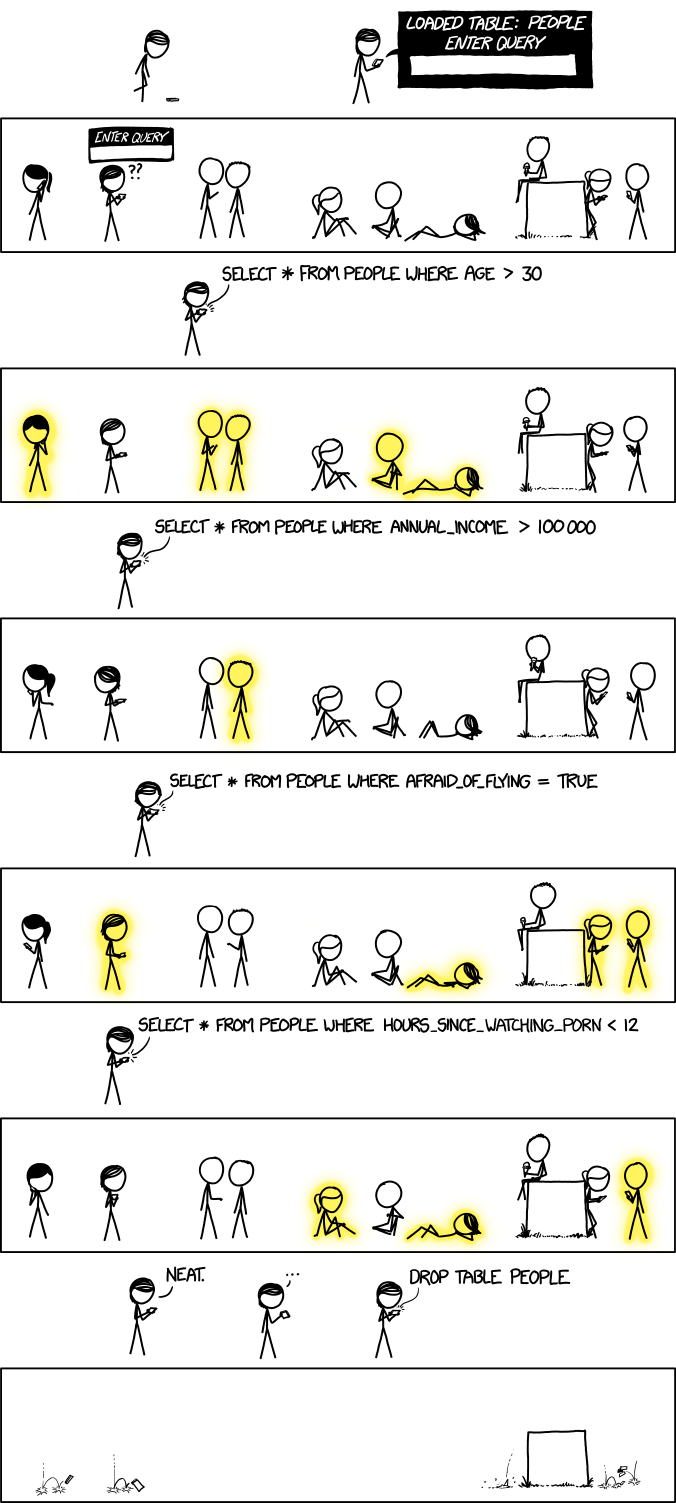
\includegraphics[width=0.7\textwidth,height=\textheight]{Images/query.png}
\caption{\href{https://www.explainxkcd.com/wiki/index.php/1409:_Query}{XKCD
1409 =\textgreater{} SQL en route pour la terminale !}}
\end{figure}

\end{document}
